\documentclass[fontsize=12pt,paper=a4,twoside]{scrartcl}
\usepackage{longtable} 
\usepackage{graphicx}
% SWP-Präambel
% C 2003-2017 Sebastian Offermann, Rainer Koschke, Karsten Hölscher
% In Zeilen 40 und 41 sind jeweils die aktuellen Daten einzutragen

\usepackage[utf8]{inputenc}     % Kodierung der Tex-Datei
\usepackage[T1]{fontenc}        % Korrekte Ausgabe von Sonderzeichen (Umlaute)
\usepackage[ngerman]{babel}     % Deutsche Einstellungen [ab \begin{document}]

\usepackage{bibgerm}            % Bibliographie
\usepackage{fancyhdr}           % obere Seitenränder gestalten
\usepackage{float}              % Floats Objekte mit [H] festsetzen
\usepackage{graphicx}           % Graphiken als jpg, png etc. einbinden
\usepackage{moreverb}           % zusätzliche verbatim-Umgebungen
\usepackage{pdflscape}          % PDF-Support für landscape
\usepackage[final]{pdfpages}    % Externe PDFs einbinden
\usepackage{stmaryrd}           % zusätzliche Symbole
\usepackage{supertabular}       % Tabellen über Seitenränder hinaus
\usepackage{tabularx}           % Tabellen mit vorgegebener Breite
\usepackage{url}                % setzt URLs schön mit \url{http://bla.laber.com/~mypage}

%%% Die Reihenfolge der folgenden Pakete muss beibehalten werden:
%%% varioref, hyperref, cleveref, bookmark
% Verweise innerhalb des Dokuments schick mit " ... auf Seite ... "
% automatisch versehen. Dazu \vref{labelname} benutzen
\usepackage[ngerman]{varioref}  % [vor hyperref für korrekte Verweise]
\usepackage[colorlinks=true, pdfstartview=FitV, linkcolor=blue,
            citecolor=blue, urlcolor=blue, hyperfigures=true,
            pdftex=true]{hyperref} % [vor bookmark wegen der Optionen]
\usepackage[ngerman]{cleveref}
\usepackage{bookmark}

\hyphenation{Arbeits-paket}     % Trennungsregeln

%%% Definitionen
\newcommand{\grad}{\ensuremath{^{\circ}} }
\renewcommand{\strut}{\vrule width 0pt height5mm depth2mm}
\newcommand{\gq}[1]{\glqq{}#1\grqq{}}

%%% Semesterkonstanten
\newboolean{langversion} %Deklaration
\setboolean{langversion}{true} %Zuweisung ist 'false' für Blockkurs
\newcommand{\jahr}[1]{2020} %2017/2018

% erstes Argument: SWP-2, zweites SWP-1
\newcommand{\highlight}[1]{\textcolor{blue}{\textbf{#1}}}
\newcommand{\variante}[2]{\ifthenelse{\boolean{langversion}}{#1}{#2}}
\newcommand{\nurlangversion}[0]%
    {\variante{\highlight{}}%Muss in SWP-2 ausgefüllt werden}}%
              {\highlight{Entfällt in SWP-1}}}
\newcommand{\swp}[0]{Software-Projekt \variante{2}{1}}
\newcommand{\semester}[0]{SoSe \jahr}

%%% Formatierungsanpassungen
% Damit Latex nicht zu lange Zeilen produziert:
\sloppy
%Uneinheitlicher unterer Seitenrand:
%\raggedbottom

% Kein Erstzeileneinzug beim Absatzanfang
% Sieht aber nur gut aus, wenn man zwischen Absätzen viel Platz einbaut
\setlength{\parindent}{0ex}

% Abstand zwischen zwei Absätzen
\setlength{\parskip}{1ex}

% Seitenränder für Korrekturen verändern
\addtolength{\evensidemargin}{-1cm}
\addtolength{\oddsidemargin}{1cm}

\bibliographystyle{gerapali}

% 1. Parameter: Euer/Eure TutorIn, z. B. {Kim Harrison}
% 2. Parameter: Abgabedatum, z. B. {05. April 2063}
% 3. Parameter: Versionsnummer, z. B. {1.1}
% 4.-9. Parameter: jeweils Name und (Uni-)Email-Adresse jedes 
%                 Gruppenmitglieds; mit einem & getrennt, z. B.
% {Robin Cowl & roco@tzi.de}
% Besteht die Gruppe aus weniger als 6 Personen, so werden die 
% übrigen Parameter leer gelassen: {}
\newcommand \swpdocument[9] {
% Lustige Header auf den Seiten
  \pagestyle{fancy}
  \setlength{\headheight}{70.55003pt}
  \fancyhead{}
  \fancyhead[LO,RE]{\swp{}\\%
                    \semester{}\\%
                    \documentTitle}
  \fancyhead[LE,RO]{Seite \thepage\\%
                    \slshape \leftmark\\%
                    \slshape \rightmark}

% Lustige Header nur auf dieser Seite (Titelseite)
  \thispagestyle{fancy}
  \fancyhead[LO,RE]{ }
  \fancyhead[LE,RO]{Universität Bremen\\%
                    FB 3 -- Informatik\\%
                    Dr. Karsten Hölscher\\%
                    TutorIn: #1}
  \fancyfoot[C]{}

% Start Titelseite
  \vspace{3cm}
  \begin{minipage}[H]{\textwidth}
    \begin{center}
      \bfseries \Large \swp{} -- \semester{}\\
      \smallskip
      \small VAK 03-BA-901.02\\
      \vspace{3cm}
    \end{center}
  \end{minipage}
  \begin{minipage}[H]{\textwidth}
    \begin{center}
      \vspace{1cm}
      \bfseries \Large \documentTitle\\
      \vfill
    \end{center}
  \end{minipage}
  \vfill
  \begin{minipage}[H]{\textwidth}
    \begin{center}
      \sffamily
      \begin{tabular}{lr}
        #4 \\
        #5 \\
        #6 \\
        #7 \\
        #8 \\
        #9 \\
      \end{tabular}
      \\[22mm]
      \itshape Abgabe: #2 --- Version #3 \\ ~
    \end{center}
  \end{minipage}
% Ende Titelseite

% Start Inhaltsverzeichnis
\newpage
  \thispagestyle{fancy}
  \fancyhead{}
  \fancyhead[LO,RE]{\swp{}\\%
                    \semester{}\\%
                    \documentTitle}
  \fancyhead[LE,RO]{Seite \thepage\\%
                    \slshape \leftmark\\~}
  \fancyfoot{}
  \renewcommand{\headrulewidth}{0.4pt}
  \tableofcontents
% Ende Inhaltsverzeichnis

% Header für alle weiteren Seiten
\newpage
  \fancyhead[LE,RO]{Seite \thepage\\%
                    \slshape \leftmark\\%
                    \slshape \rightmark}

}



%
% Und jetzt geht das Dokument los....
%
\begin{document}
\newcommand\documentTitle{Benutzerhandbuch}
 %\begin{minipage}[b]{\textwidth}
 \vspace{1mm}
 \begin{figure}[!b]
  \centering
  
\includegraphics[width=0.5\textwidth]{pics/SpaceStudioLogo.png}\\
\end{figure}

\swpdocument{Dr. Karsten Hölscher}{02. August 2020}{1.1}%
            {Clara Maria Odinius & odinius@uni-bremen.de}%
            {Habib Mergan & habib1@uni-bremen.de}%
            {Kevin Santiago Rey Rodriguez & kev\_rey@uni-bremen.de}%
            {Liam Hurwitz & hurwitz@uni-bremen.de}%
            {Mehmet Ali Baykara & baykara@uni-bremen.de}%
            {Miguel Alejandro Caceres Pedraza & mcaceres@uni-bremen.de}%

%%%%%%%%%%%%%%%%%%%%%%%%%%%%%%%%%%%%%%%%%%%%%%%%%%%%%%%%%%%%%%%%%%%%%%%%



%%%%%%%%%%%%%%%%%%%%%%%%%%%%%%%%%%%%%%%%%%%%%%%%%%%%%%%%%%%%%%%%%%%%%%%%
\section{Einführung}

Willkommen bei Spacestudio Game\\
Dieser Benutzerhandbuch beschreibt wie die Software bzw. das Spiel gespielt wird und darüberhinaus dient als Anleitung für das Programm. Bitte lesen Sie sich dieses Handbuch durch bevor Sie die Anwendung starten. Nach aufmerksamtiges Lesen des Handbuchs werden Sie alle Funktionalität des Spiels erfahren und verstehen wie Sie mit dem Spiel umgehen können.

Das Spiel ist ein erweiterte Version des Faster Than Light, daher werden Sie viel gemeinsamkeite zwischen das Spiel und FTL. 

%%%%%%%%%%%%%%%%%%%%%%%%%%%%%%%%%%%%%%%%%%%%%%%%%%%%%%%%%%%%%%%%%%%%%%%%
\subsection{Zweck}

Das Handbuch ist im Rahmen vom ReSWP 2 SOSE20 von der Gruppe SpaceStudio geschrieben. Der Zweck dieses Handbuches besteht darin, eine Anleitungzu der Verwendung von SpaceStudio bereitzustellen.

%%%%%%%%%%%%%%%%%%%%%%%%%%%%%%%%%%%%%%%%%%%%%%%%%%%%%%%%%%%%%%%%%%%%%%%%

\section{Installation}
In diesem Abschnitt wird beschieben, wie das Programm installiert wird und entsprechende Systemvoraussetzungen aufgelistet.

\subsection{Systemvoraussetzungen}
1. Java 11 oder höher \\
2. Windows 10, macOS, Linux \\
3. Gradle 5.2 oder höher \\
4. Spring Boot 2.0.3.RELEASE \\
5.  Spring Framework 5.0.7.RELEASE or höher. \\
6. 1920X1080 Auflösung
 

\subsection{Installationsschritte}
Folgende  Schritte sind für Installation benötigt. \\
1. Nach dem Sie alle benötigte tools, die in Systemvoraussetzungen aufgelistet wurden, installiert haben, starten \\
2. Starten Sie der Server und warten Sie bis der Server hochfährt ca 1 Minute\\
3. Wenn der Server gestartet hat, dann starten Sie Client

 


%%%%%%%%%%%%%%%%%%%%%%%%%%%%%%%%%%%%%%%%%%%%%%%%%%%%%%%%%%%%%%%%%%%%%%%%

\section{Start}
In diesem Abschnitt wird komplett Anleitung der Spiel beschrieben. Alle notwendige Schritte werden mit entsprechendem Bild gezeigt. Wenn 
\subsection{Anmeldung}
\begin{figure}[htp]
%%	\centering
	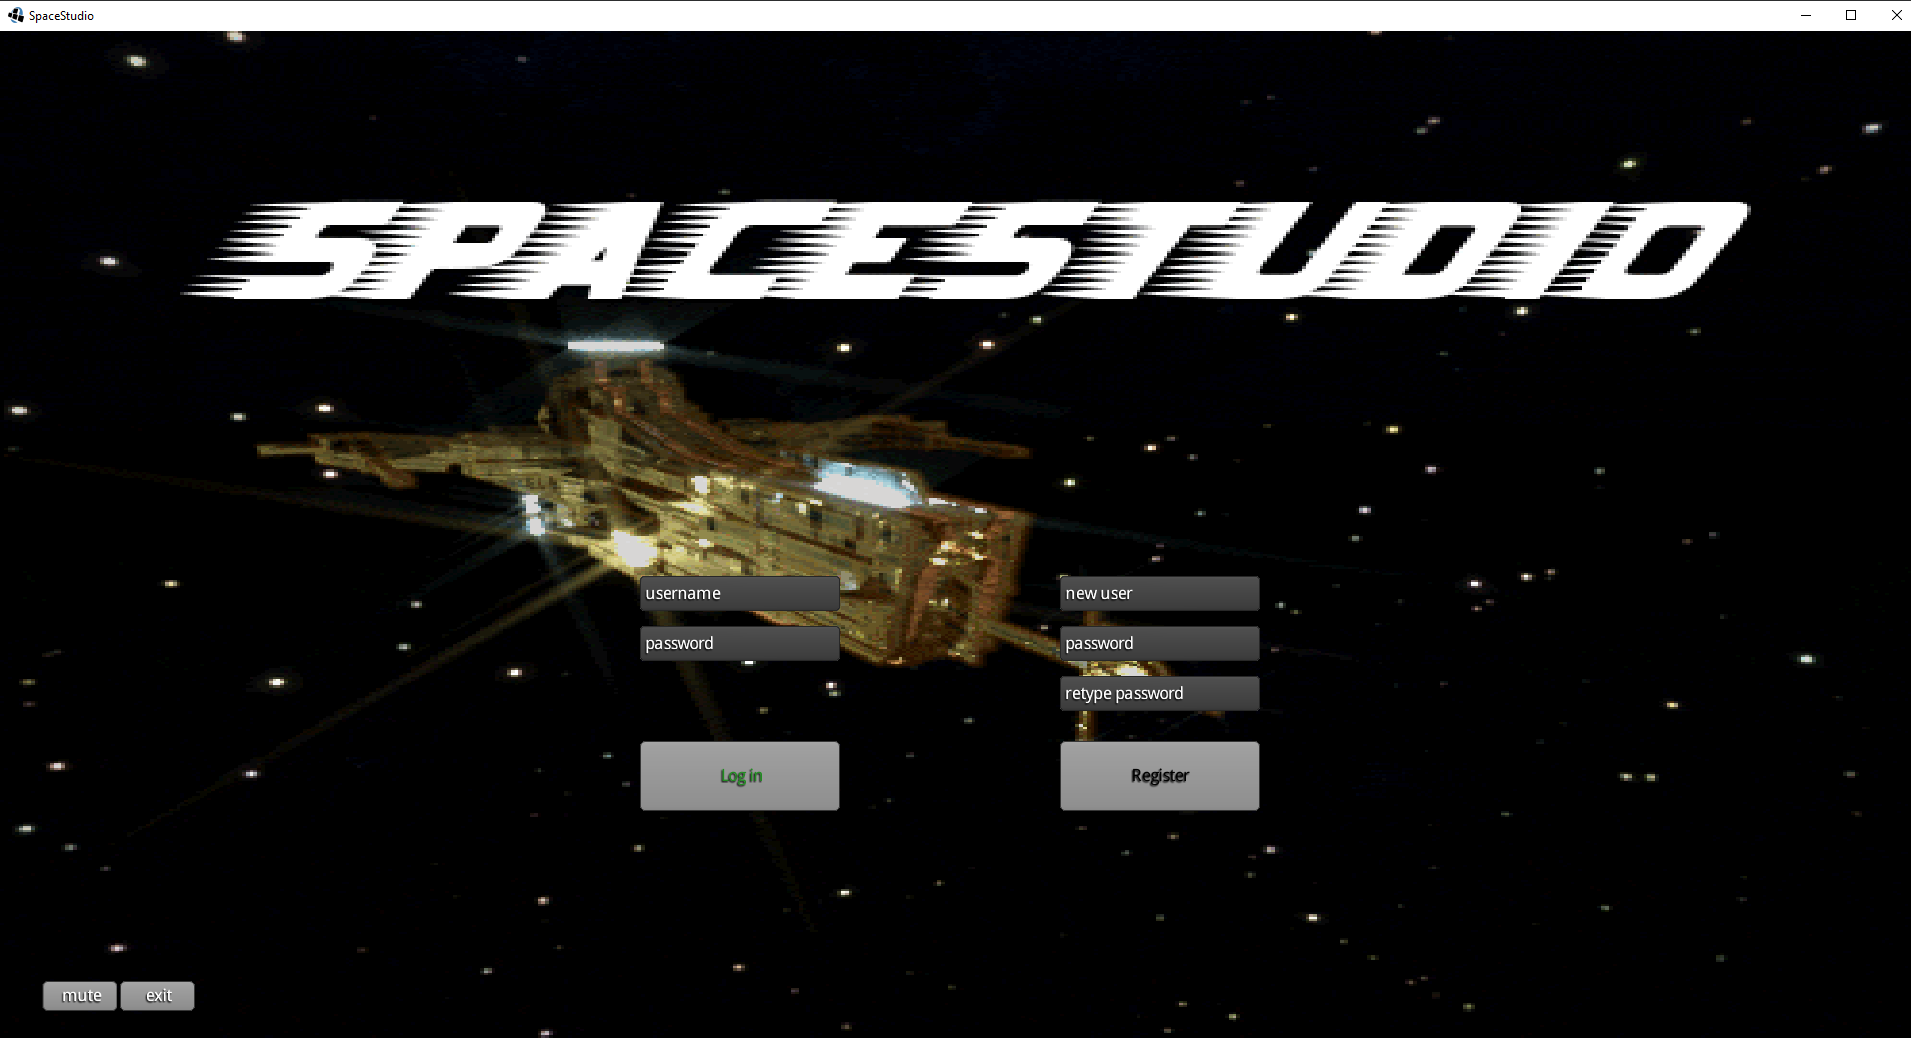
\includegraphics[width=1.00\linewidth]{pics/loginscreen.png}
	\caption{Anmeldung}
	\label{fig1}
\end{figure}
Die Loginseite ermöglicht, dass man ein Profil erstellen kann und sich mit erzeugter Profil jeder Zeit beim Spiel einlogen bzw. auslogen kann. Beim Start des Spiels muss man ein Benutzername und ein Password eingeben, wenn eingegebene Benutzername nicht vergegeben ist dann wird als neue Profil angelegt. Nach erfolgreiche Anmeldung bzw. Registrierung kann man sich mit entspechende Anmeldedaten anmelden. Geben Sie Ihre persönliche Benutzername und Password auf der linken Seite ein. Nach validierung Anmeldedaten werden Sie nächste Bildschirm bzw. zum Menu weitergeleitet. 

Auf der unten linken ester Bildschirm sieht man zwei Buttons nämlich mute und exit. Der Mute-Knopf ist dafür da, dass man hinter Grundmusik an- und ausschalten kann. Mit Exit-Knopf kann man das Spiel ohne weiteres beenden.

\newpage

%%%%%%%%%%%%%%%%%%%%%%%%%%%%%%%%%%%%%%%%%%%%%%%%%%%%%%%%%%%%%%%%%%%%%%%%
\subsection{Menu}

\begin{figure}[htp]
	\centering
	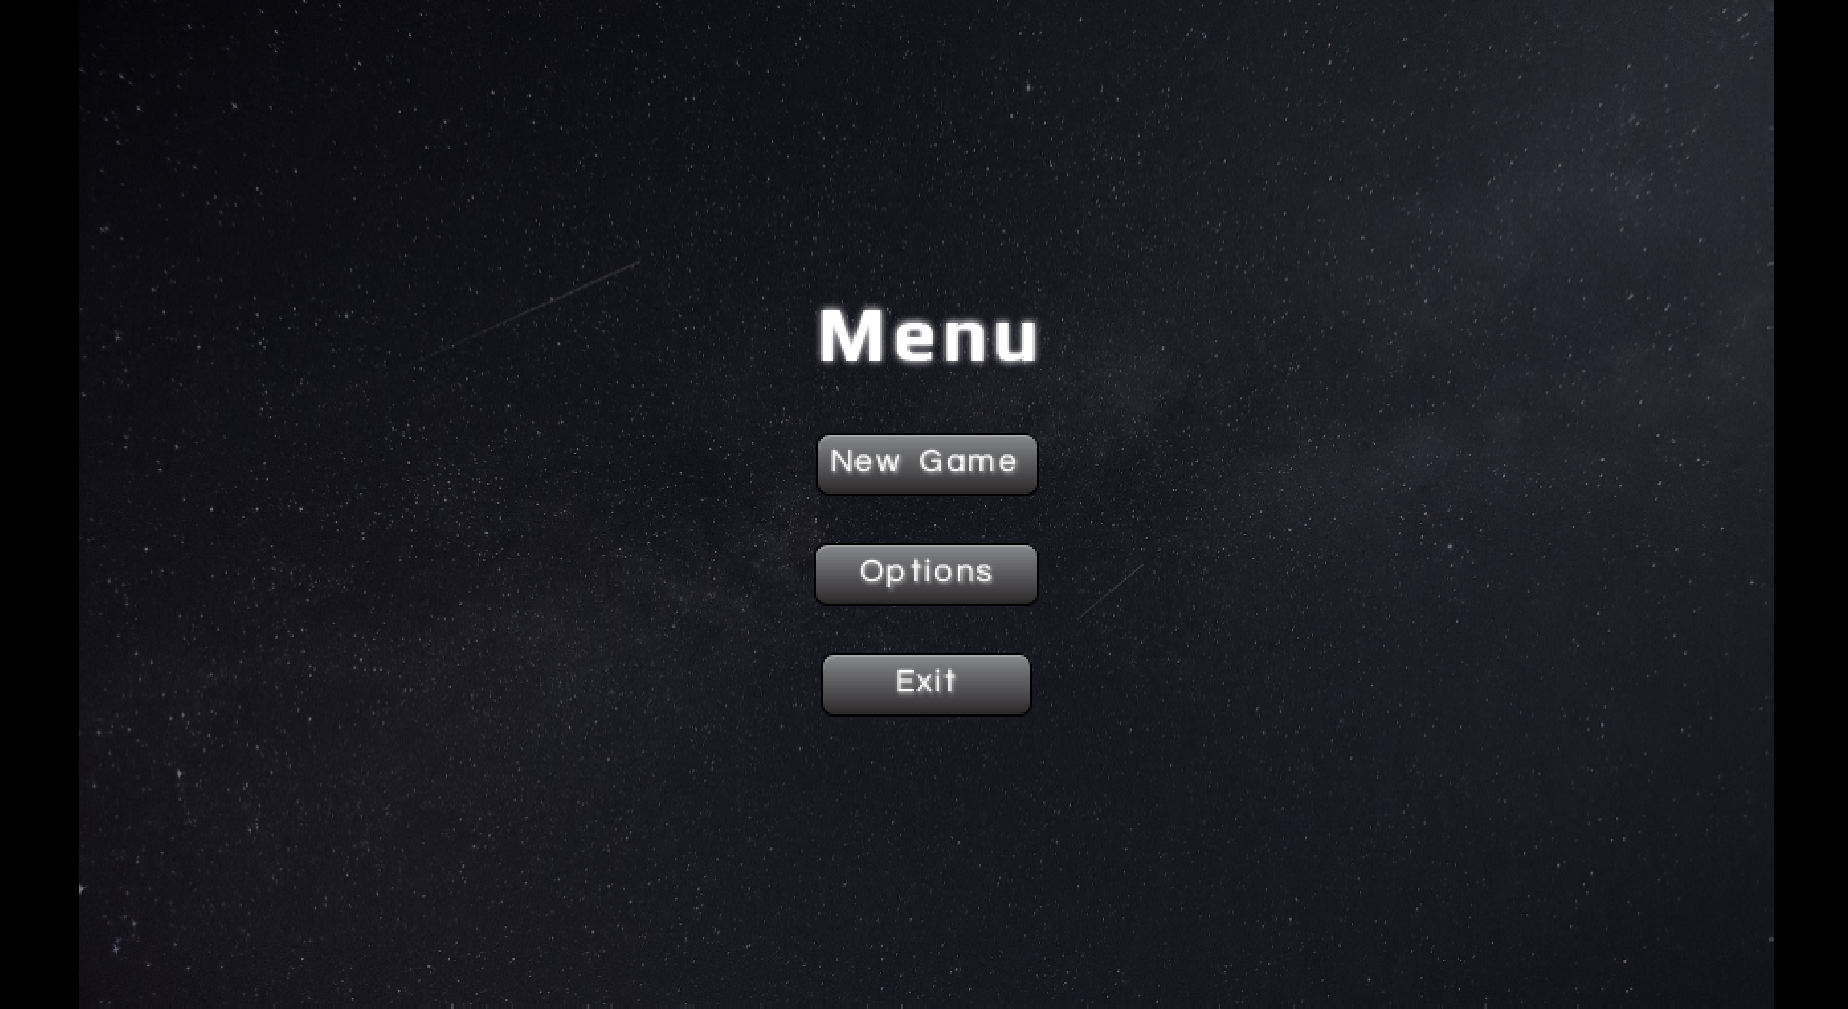
\includegraphics[width=1.00\linewidth]{pics/menuscreen.png}
	\caption{Menu}
	\label{fig1}

\end{figure}
Falls Sie sich erfolgreich eingelogt haben, werden Sie auf Menuseite weitergleitet. Hier sehen Sie drei Knöpfe:
New Game ist für neues Spiel anzufangen. \\
Options ist zurzeit nicht verfügbar, allerdings sollte für persönliche Anpassungen implementiert werden. \\
Exit ist für Beendung des Spiels.\\
Falls Sie bereits angemeldeter Benutzer sind, werden Sie ein weiteres Knopf sehen nämlich: \\
Continue dient dafür ein untergebroche Spiel fortzusetzen.
\newpage
%%%%%%%%%%%%%%%%%%%%%%%%%%%%%%%%%%%%%%%%%%%%%%%%%%%%%%%%%%%%%%%%%%%%%%%%
\subsection{Spielmodus}
\begin{figure}[htp]
	\centering
	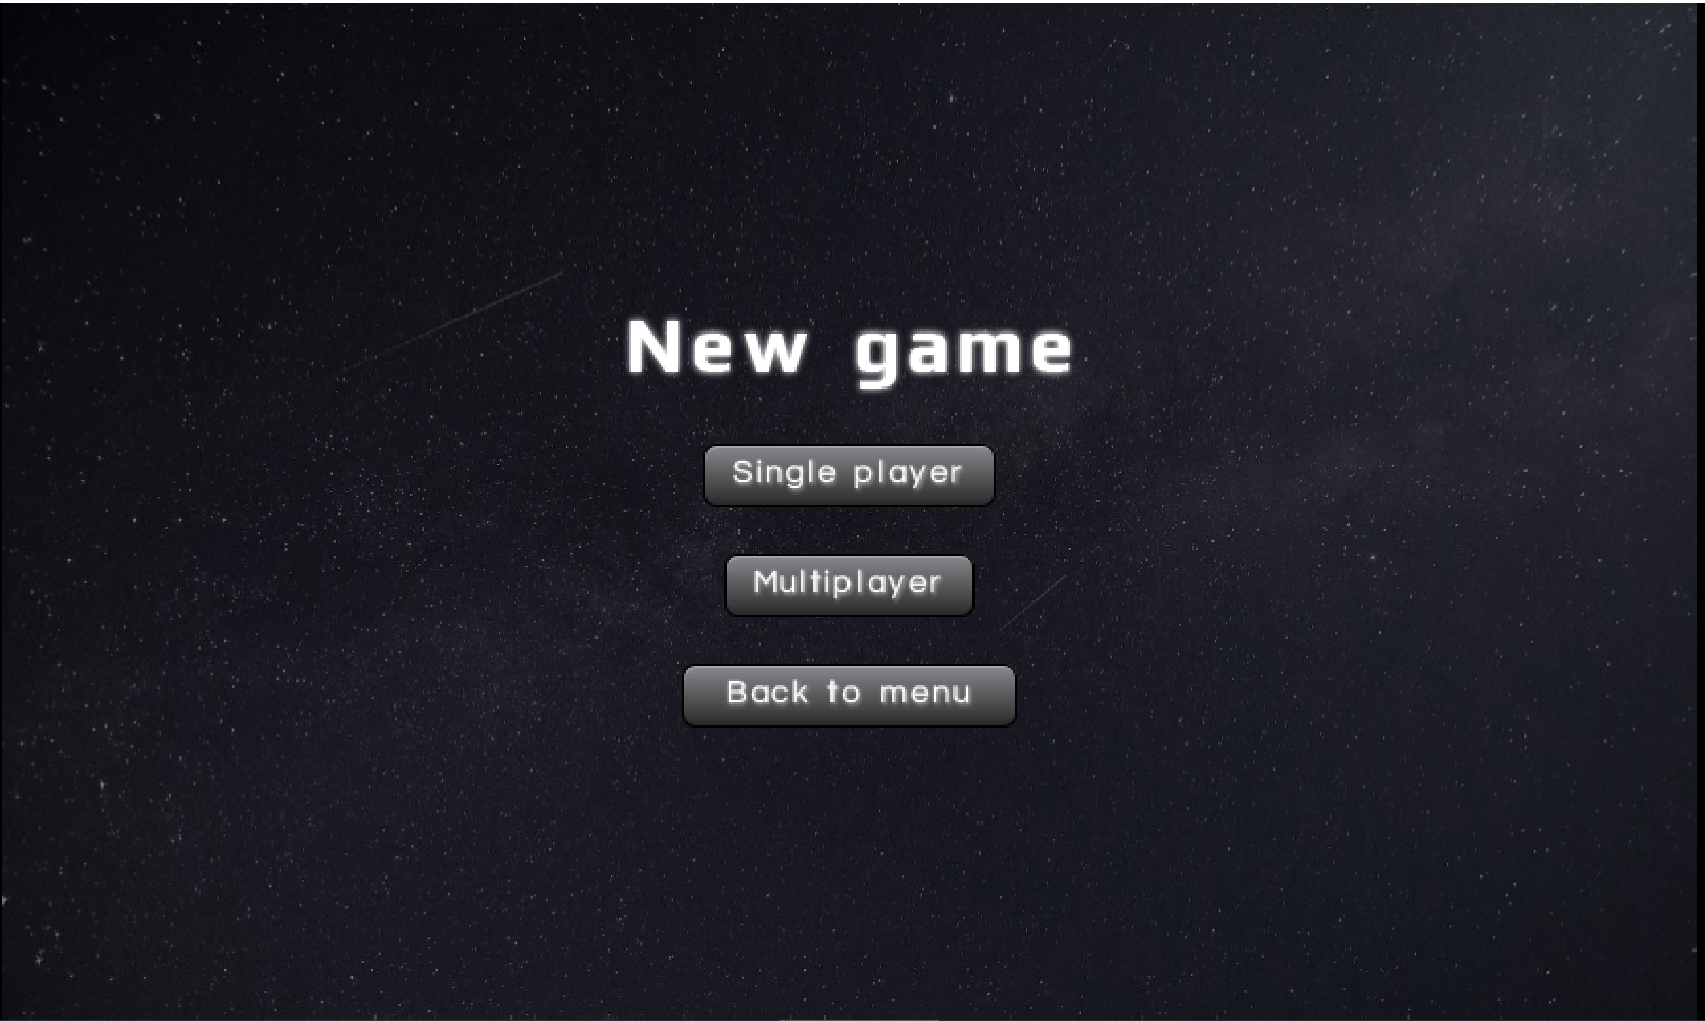
\includegraphics[width=1.00\linewidth]{pics/gamemodescreen.png}
	\caption{Spielmodus}
	\label{fig1}
\end{figure}
\newpage
Ein weiteres Bildschirm ist Gamemodussscreen, wo man Spielmodus aus wählen oder wiederzurück zu vorherige Seit kehren kann. Single player modus ermöglicht Spieler wenn kein weiteres Spieler da ist und trotzdem spielen zu können. In diesem Fall wird der Gegner duch KI realisiert und der Spiel kann ohne problem mit der Computer spielen. Single playermodus sieht es folgendes:
\begin{figure}[htp]
	\centering
	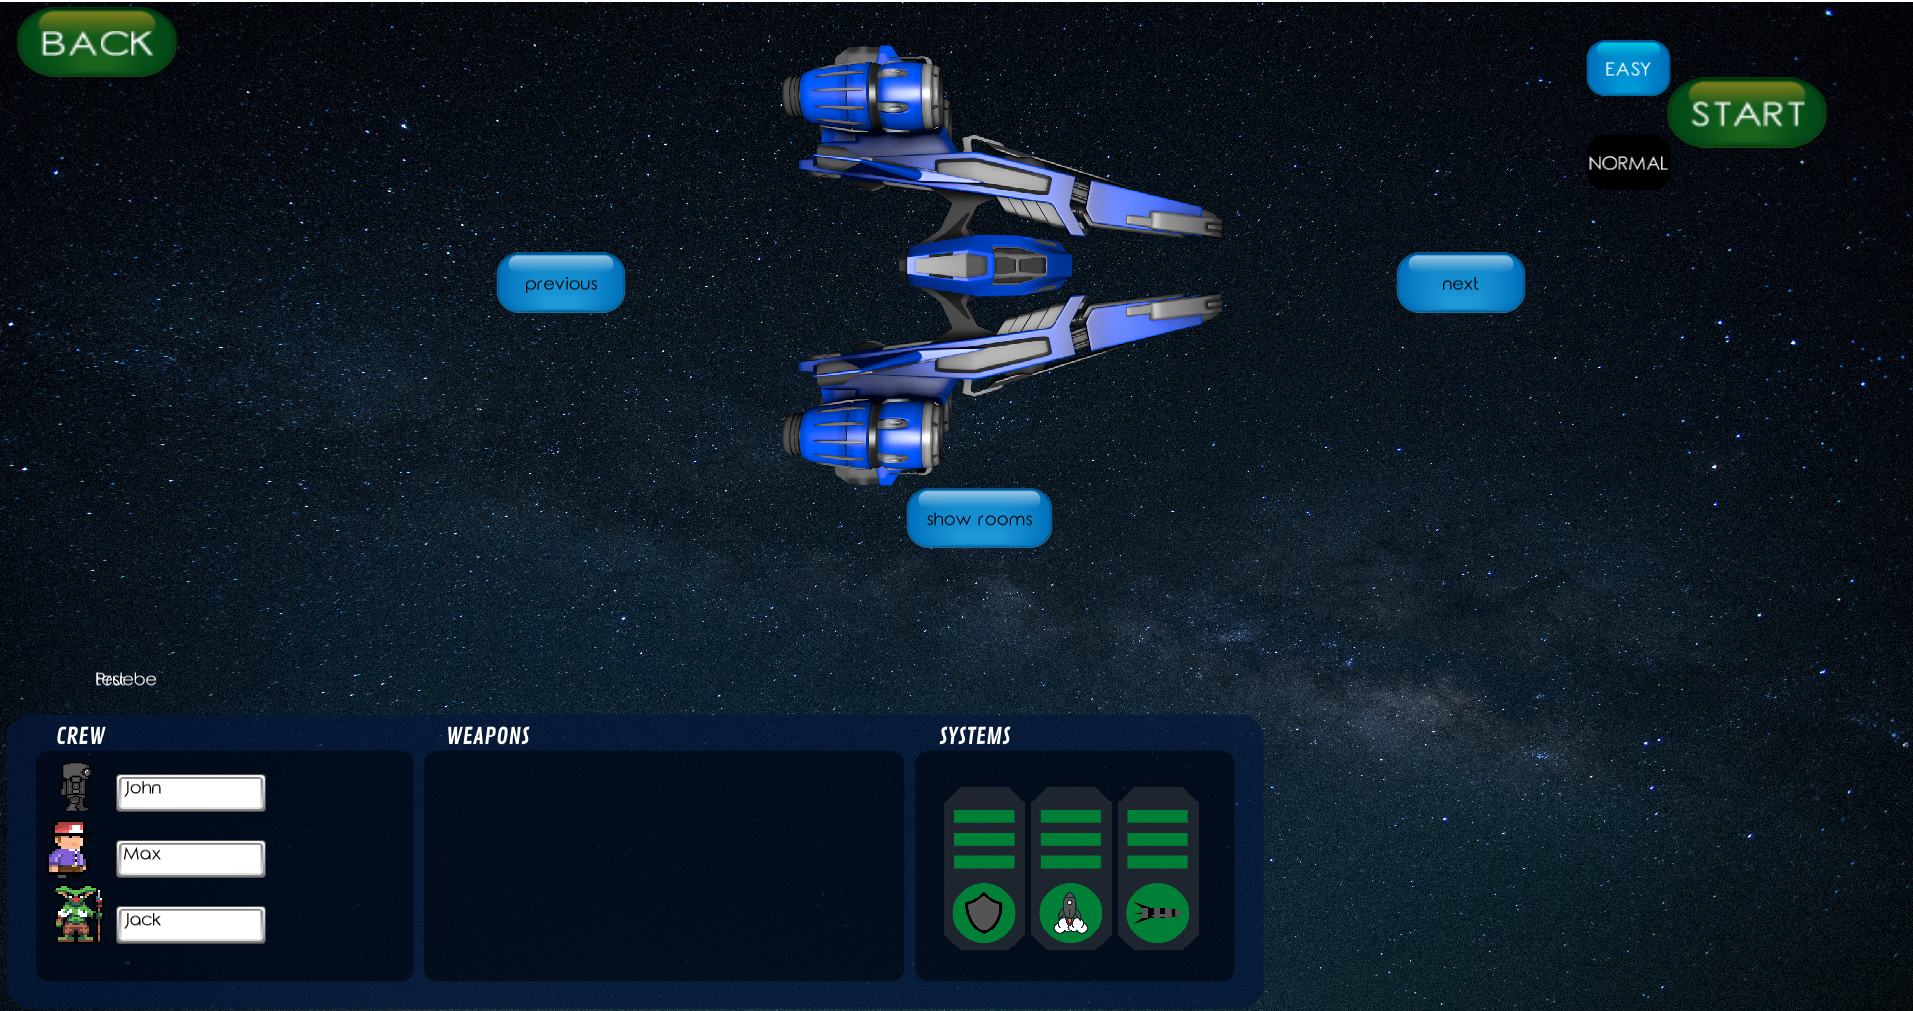
\includegraphics[width=1.00\linewidth]{pics/singleplayerscreen.png}
	\caption{Spielmodus}
	\label{fig1}
\end{figure}
\newpage
 In Multiplayer modus kann man mit andere online Spieler spielen, dh. wenn zwei Spieler auf gleichen Server angemeldet sind, dann kann man gegenseitig spielen.  
\newpage
%%%%%%%%%%%%%%%%%%%%%%%%%%%%%%%%%%%%%%%%%%%%%%%%%%%%%%%%%%%%%%%%%%%%%%%%
\subsection{Raumschiff Auswahl}
Beschreibung der Spielmodus.
%%%%%%%%%%%%%%%%%%%%%%%%%%%%%%%%%%%%%%%%%%%%%%%%%%%%%%%%%%%%%%%%%%%%%%%%
\subsection{Map}
Beschreibung der Spielmodus.

%%%%%%%%%%%%%%%%%%%%%%%%%%%%%%%%%%%%%%%%%%%%%%%%%%%%%%%%%%%%%%%%%%%%%%%%
\section{Eigentliches Spiel}
Beschreibung der Kamfscreen.
%%%%%%%%%%%%%%%%%%%%%%%%%%%%%%%%%%%%%%%%%%%%%%%%%%%%%%%%%%%%%%%%%%%%%%%%
\subsection{Spiel Verlauf}
Beschreibung der Spielmodus.
%%%%%%%%%%%%%%%%%%%%%%%%%%%%%%%%%%%%%%%%%%%%%%%%%%%%%%%%%%%%%%%%%%%%%%%%

\subsection{Spiel Unterbrechung}
Beschreibung der Unterbrechung des Spiels und fortsetzen.
%%%%%%%%%%%%%%%%%%%%%%%%%%%%%%%%%%%%%%%%%%%%%%%%%%%%%%%%%%%%%%%%%%%%%%%%


\subsection{Spiel Wiedergeben}
Spielzüge detaliert wiedergeben
\end{document}

%%% Local Variables: 
%%% mode: latex
%%% mode: reftex
%%% mode: flyspell
%%% ispell-local-dictionary: "de_DE"
%%% TeX-master: t
%%% End: 
